\documentclass[a4paper]{article}
\usepackage[utf8]{inputenc}
\usepackage[margin=1in]{geometry}
\usepackage{amsmath}
\usepackage{amssymb}
\usepackage{setspace}
\usepackage{graphicx}



\title{Chapter 5\\Differentiation}
\author{solutions by Hikari}
\date{December 2021}

\begin{document}

\newcommand{\V}{\mathbf}

\maketitle

\paragraph{1.}
\[
\phi(y)=\left|\frac{f(x)-f(y)}{x-y} \right|\leq |x-y|
\]
$|x-y|\to0$ as $y\to x$, so $\phi(y)\to0$ as $y\to x$, which means $f'(x)=0$. By Theorem 5.11, $f$ is constant.

\paragraph{2.}
For $x_1,x_2\in(a,b)$ and $x_2>x_1$, there exists $x\in(x_1,x_2)$ such that $f(x_2)-f(x_1)=(x_2-x_1)f'(x)$, and since $f'(x)>0$,\; $f(x_2)-f(x_1)>0$. So $f$ is strictly increasing in $(a,b)$, and therefore the inverse function $g$ exists.

Let $x,t\in(a,b)$, and $y=f(x),\,u=f(t)$. Then
\[
\phi(u)=\frac{g(u)-g(y)}{u-y}=\frac{t-x}{f(t)-f(x)}=\frac{1}{\frac{f(t)-f(x)}{t-x}}\to\frac{1}{f'(x)}
\]
when $t\to x$, which means for every $\varepsilon>0$ there is $\delta'>0$ such that $|t-x|<\delta'$ implies $|\phi(u)-\frac{1}{f'(x)}|<\varepsilon$.\; $f$ is a continuous 1-1 mapping of the compact metric space $[a',b']$ where $a<a'<b'<b$, so $g=f^{-1}$ is a continuous mapping by Theorem 4.17. So for $\delta'>0$ there is $\delta>0$ such that $|u-y|<\delta$ implies $|g(u)-g(y)|=|t-x|<\delta'$ and therefore $|\phi(u)-\frac{1}{f'(x)}|<\varepsilon$, so
\[
g'(f(x))=g'(y)=\lim_{u\to y}\phi(u)=\frac{1}{f'(x)}
\]

\paragraph{3.}
Let $\varepsilon<\frac{1}{M}$, then $f'(x)=1+\varepsilon g'(x)>1-\frac{1}{M}\cdot M=0$, so by Exercise 2, $f$ is strictly increasing and therefore one-to-one.

\paragraph{4.}
Consider the function
\[
f(x)=C_0x+\frac{C_1}{2}x^2+\cdots+\frac{C_{n-1}}{n}x^n+\frac{C_n}{n+1}x^{n+1}
\]
which is differential. $f(0)=f(1)=0$, so by Theorem 5.10, there is a $x\in(0,1)$ such that
\[
f'(x)=C_0+C_1x+\cdots+C_{n-1}x^{n-1}+C_nx^n=0
\]

\paragraph{5.}
For every $\varepsilon>0$, there is a $x_0$ such that $x>x_0$ implies $|f'(x)|<\varepsilon$, then for $x>x_0$, there is a $x_1\in(x,x+1)$ such that
\[
|g(x)|=\left|\frac{f(x+1)-f(x)}{x+1-x} \right|=|f'(x_1)|<\varepsilon
\]
so $g(x)\to0$ as $x\to+\infty$.

\paragraph{6.}
\[
g'(x)=\frac{f'(x)}{x}-\frac{f(x)}{x^2}=\frac{1}{x}\left(f'(x)-\frac{f(x)-f(0)}{x-0} \right)=\frac{1}{x}\left(f'(x)-f'(x_1) \right)>0
\]
where $0<x_1<x$, so $f'(x)>f'(x_1)$. By Theorem 5.11,\; $g$ is monotonically increasing.

\paragraph{7.}
\[
\lim_{t\to x}\frac{f(t)}{g(t)}=\lim_{t\to x}\frac{\frac{f(t)-f(x)}{t-x}}{\frac{g(t)-g(x)}{t-x}}=\frac{\lim_{t\to x}\frac{f(t)-f(x)}{t-x}}{\lim_{t\to x}\frac{g(t)-g(x)}{t-x}}=\frac{f'(x)}{g'(x)}
\]

\paragraph{8.}
$f'$ is continuous on the compact metric space $[a,b]$, so it is uniformly continuous by Theorem 4.19. For every $\varepsilon>0$, there is $\delta>0$ such that $x,y\in[a,b]$ and $|y-x|<\delta$ implies $|f'(y)-f'(x)|<\varepsilon$, then for $x,t\in[a,b]$ and $0<|t-x|<\delta$, there is a $p$ between $x$ and $t$ such that
\[
\left|\frac{f(t)-f(x)}{t-x}-f'(x) \right|=\left|f'(p)-f'(x) \right|<\varepsilon
\]
since $|p-x|<|t-x|<\delta$. The results hold for vector-valued functions with arbitrary dimension $k$ since for the $i$-th component, we can find $\delta_i$ such that
\[
\left|\frac{f_i(t)-f_i(x)}{t-x}-f_i'(x) \right|<\frac{\varepsilon}{\sqrt{k}}
\]
when $0<|t-x|<\delta_i$, then for $|t-x|<\delta=\min(\delta_1,\delta_2,\cdots,\delta_k)$, 
\[
\left|\frac{\V{f}(t)-\V{f}(x)}{t-x}-\V{f}'(x) \right|<\sqrt{\left(\frac{\varepsilon}{\sqrt{k}} \right)^2\cdot k}=\varepsilon
\]

\paragraph{9.}
For every $t$ there is a $u\in(0,t)$ or $(t,0)$ such that
\[
\frac{f(t)-f(0)}{t-0}=f'(u)
\]
Then
\[
\lim_{t\to0}\frac{f(t)-f(0)}{t-0}=\lim_{t\to0}f'(u)=3
\]
since $u\to0$ as $t\to0$. So $f'(0)=3$.

\paragraph{10.}
Let $f(x)=f_1(x)+if_2(x)$, then by Theorem 5.13,
\[
\lim_{x\to0}\frac{f(x)}{x}=\lim_{x\to0}\frac{f_1(x)}{x}+\lim_{x\to0}\frac{if_2(x)}{x}=\lim_{x\to0}f_1'(x)+\lim_{x\to0}if_2'(x)=\lim_{x\to0}f(x)=A
\]
Similarly $\lim_{x\to0}\frac{g(x)}{x}=B$. Therefore,
\[
\lim_{x\to0}\frac{f(x)}{g(x)}=\left\{\lim_{x\to0}\frac{f(x)}{x}-A \right\}\cdot\lim_{x\to0}\frac{x}{g(x)}+A\cdot\lim_{x\to0}\frac{x}{g(x)}=\{A-A\}\cdot\frac{1}{B}+A\cdot\frac{1}{B}=\frac{A}{B}
\]

\paragraph{11.}
\[
f''(x)=\frac{f''(x)}{2}+\frac{f''(x)}{2}=\frac{1}{2}\lim_{h\to0}\frac{f'(x+h)-f'(x)}{h}+\frac{1}{2}\lim_{h\to0}\frac{f'(x-h)-f'(x)}{-h}=\lim_{h\to0}\frac{f'(x+h)-f'(x-h)}{2h}
\]
$f''(x)$ exists, so $f'(x)$ exists in a neighborhood of $x$, which means $f(x)$ is differentiable in the neighborhood. Let $A(h)=f(x+h)+f(x-h)-2f(x)$,\; $B(h)=h^2$, then $A(h)$ is differentiable in a neighborhood of $h=0$ with $A'(h)=f'(x+h)-f'(x-h)$, and $B(h)$ is differentiable in a neighborhood of $h=0$ with $B'(h)=2h$. As $h\to0$,\; $A(h)\to0$ and $B(h)\to0$, so by Theorem 5.13,
\[
\lim_{h\to0}\frac{f(x+h)+f(x-h)-2f(x)}{h^2}=\lim_{h\to0}\frac{A(h)}{B(h)}=\lim_{h\to0}\frac{A'(h)}{B'(h)}=\lim_{h\to0}\frac{f'(x+h)-f'(x-h)}{2h}=f''(x)
\]
Let $f$ be such that
\[
f(x)=
\begin{cases}
1,\quad & x>0\\
0,\quad & x=0\\
-1,\quad & x<0
\end{cases}
\]
then 
\[
\lim_{h\to0}\frac{f(0+h)+f(0-h)-2f(0)}{h^2}=0
\]
while $f'(0)$ and $f''(0)$ do not exist.

\paragraph{12.}
For $x>0$,\; $f(x)=x^3$,\; $f'(x)=3x^2$,\; $f''(x)=6x$,\; $f^{(3)}(x)=6$. For $x<0$,\; $f(x)=-x^3$,\; $f'(x)=-3x^2$,\; $f''(x)=-6x$,\; $f^{(3)}(x)=-6$. For $x=0$,
\[
f'(0)=\lim_{t\to0}\frac{f(t)-f(0)}{t-0}=\lim_{t\to0}f'(p)=\lim_{p\to0}\pm 3p^2=0
\]
where $p\in(0,t)$ or $(t,0)$.
\[
f''(0)=\lim_{t\to0}\frac{f'(t)-f'(0)}{t-0}=\lim_{t\to0}f''(q)=\lim_{q\to0}\pm6q=0
\]
where $q\in(0,t)$ or $(t,0)$.
\[
f^{(3)}(0+)=6,\qquad f^{(3)}(0-)=-6
\]
so $f^{(3)}(0)$ does not exist.

\paragraph{13.}
$f$ is a complex function since $x^a$ may be complex for $x<0$. Assume the derivative laws of real functions holds for complex functions.
\medskip

(a)
$f$ is continuous for all $x\neq0$. At $x=0$,\; $f$ is continuous if and only if $\lim_{t\to0}f(t)=f(0)$. If $a\leq0$,\; $\lim_{t\to0}f(t)$ does not exist. If $a>0$,\; $\lim_{t\to0}f(t)=0=f(0)$.
\medskip

(b)
\[
f'(0)=\lim_{t\to0}\frac{f(t)-f(0)}{t-0}=\lim_{t\to0}t^{a-1}\sin(|x|^{-c})
\]
If $a\leq1$, the limit does not exist. If $a>1$, the limit exists and is equal to $0$.
\medskip

(c)
For $x\neq0$,
\[
f'(x)=ax^{a-1}\sin(|x|^{-c})-cx^{a+1}|x|^{-c-2}\cos(|x|^{-c})
\]
If $a<1+c$, consider $x>0$ and $|x|^{-c}=2n\pi$ where $n$ is an integer, then
\[
f'(x)=-cx^{a-c-1}\to\infty
\]
as $x\to0$, so $f'$ is not bounded.

If $a\geq 1+c$, then
\[
|f'(x)|\leq|a||x|^{a-1}+c|x|^{a-c-1}\leq |a|+c
\]
so $f'$ is bounded.
\medskip

(d)
$f'$ is continuous for all $x\neq0$. At $x=0$,\; $f'$ is continuous if and only if $\lim_{t\to0}f'(t)=f'(0)=0$.

If $a\leq 1+c$, consider $t>0$ and $|t|^{-c}=2n\pi$ where $n$ is an integer, then
\[
\lim_{t\to0}f'(t)=\lim_{t\to0}-c\,t^{a-c-1}=
\begin{cases}
\infty\qquad & \textit{if $a-c-1<0$}\\
-c\neq0\qquad & \textit{if $a-c-1=0$}
\end{cases}
\]
so $f'$ is not continuous.

If $a>1+c$, 
\[
\lim_{t\to0}|f'(t)|\leq \lim_{t\to0}|a||t|^{a-1}+\lim_{t\to0}c|t|^{a-c-1}=0
\]
so $\lim_{t\to0}f'(t)=0=f'(0)$.
\medskip

(e)
\[
f''(0)=\lim_{t\to0}\frac{f'(t)-f'(0)}{t-0}=\lim_{t\to0}a\,t^{a-2}\sin(|t|^{-c})-\lim_{t\to0}c\,t^{a}|t|^{-c-2}\cos(|t|^{-c})
\]

If $a\leq 2+c$, consider $t>0$, then
\[
f''(0)=\lim_{t\to0}t^{a-c-2}\left(a\,t^c\sin(t^{-c})-c\cos(t^{-c}) \right)=\lim_{t\to0}-c\,t^{a-c-2}\cos(t^{-c})
\]
which does not exist.

If $a>2+c$, then
\[
|f''(0)|\leq \lim_{t\to0}|a||t|^{a-2}+\lim_{t\to0}c|t|^{a-c-2}=0
\]
so $f''(0)=0$.
\medskip

(f)
For $x\neq0$,
\begin{equation*}
    \begin{split}
      f''(x) & =\left(a(a-1)x^{a-2}-c^2x^{a+2}|x|^{-2c-4} \right)\sin(|x|^{-c})\\  
      & +\left(-acx^a|x|^{-c-2}-c(a+1)x^a|x|^{-c-2}-c(-c-2)x^{a+2}|x|^{-c-4} \right)\cos(|x|^{-c})
    \end{split}
\end{equation*}

If $a<2+2c$, consider $x>0$ and $|x|^{-c}=(2n+\frac{1}{2})\pi$ where $n$ is an integer, then
\[
f''(x)=x^{a-2c-2}\left(a(a-1)x^{2c}-c^2 \right)\to\infty
\]
as $x\to0$, so $f''$ is not bounded.

If $a\geq 2+2c$, then
\[
|f''(x)|\leq |a(a-1)|+|c^2|+|ac|+|c(a+1)|+|c(c+2)|
\]
so $f''$ is bounded.
\medskip

(g)
$f''$ is continuous for all $x\neq0$. At $x=0$,\; $f''$ is continuous if and only if $\lim_{t\to0}f''(t)=f''(0)=0$.

If $a\leq2+2c$, consider $t>0$ and $|t|^{-c}=(2n+\frac{1}{2})\pi$ where $n$ is an integer, then
\[
\lim_{t\to0}f''(t)=\lim_{t\to0}t^{a-2c-2}\left(a(a-1)t^{2c}-c^2 \right)=\begin{cases}
\infty\qquad & \textit{if $a-2c-2<0$}\\
-c^2\neq0\qquad & \textit{if $a-2c-2=0$}
\end{cases}
\]
so $f''$ is not continuous.

If $a>2+2c$, 
\[
\lim_{t\to0}|f''(t)|\leq \lim_{t\to0}\left(|a(a-1)||t|^{a-2}+|c^2+c-2ac||t|^{a-c-2}+|c^2||t|^{a-2c-2} \right)=0
\]
so $\lim_{t\to0}f''(t)=0=f''(0)$.

\paragraph{14.}
If $f$ is convex, let $x_1,x_2$ be such that $a<x_1<x_2<b$, then by Exercise 4.23, 
\[
f'(x_1)=\lim_{t\to x_1}\frac{f(t)-f(x_1)}{t-x_1}\leq\frac{f(x_2)-f(x_1)}{x_2-x_1}\leq\lim_{t\to x_2}\frac{f(t)-f(x_2)}{t-x_2}=f'(x_2)
\]
which means $f$ is monotonically increasing.

If $f$ is monotonically increasing, let $x,y\in(a,b)$,\; $0<\lambda<1$, and $z=\lambda x+(1-\lambda)y$. Then by Theorem 5.10,
\[
\frac{f(z)-f(x)}{z-x}=f(w_1)\leq f(w_2)=\frac{f(y)-f(z)}{y-z}
\]
where $w_1\in(x,z)$ and $w_2\in(z,y)$. Rearranging,
\[
(y-x)f(z)\leq(y-z)f(x)+(z-x)f(y)
\]
\[
f(\lambda x+(1-\lambda)y)\leq \lambda f(x)+(1-\lambda)f(y)
\]
which means $f$ is convex.

$f''(x)\geq0$ if and only if $f'(x)$ is monotonically increasing, if and only if $f$ is convex.

\paragraph{15.}
For every $x\in(a,\infty)$ and $h>0$, by Taylor's theorem, 
\[
f(x+2h)=f(x)+f'(x)\cdot2h+\frac{f''(\xi)}{2}(2h)^2
\]
where $\xi\in(x,x+2h)$, so
\[
f'(x)=\frac{1}{2h}\left[f(x+2h)-f(x) \right]-hf''(\xi)
\]
\[
|f'(x)|\leq\frac{1}{2h}\left[M_0-(-M_0) \right]+hM_2=\frac{M_0}{h}+hM_2
\]
If $M_0=0$, then $M_1=0$, so $M_1^2\leq4M_0M_2$ holds. If $M_2=0$, then $M_1$ is a constant, which means $f$ is a linear function, which is bounded only if $f$ is a constant function, which means $f'(x)=0$ and $M_1=0$, so $M_1^2\leq4M_0M_2$ holds. So assume $M_0,M_2\neq0$, and let $h=\sqrt{\frac{M_0}{M_2}}$, then $|f'(x)|\leq2\sqrt{M_0M_2}$ for every $x$, so $M_1\leq2\sqrt{M_0M_2}$,\; $M_1^2\leq4M_0M_2$.

Let $f$ be such that
\[
f(x)=\begin{cases}
2x^2-1\qquad & (-1<x<0)\\
\frac{x^2-1}{x^2+1}\qquad & (0\leq x<\infty)
\end{cases}
\]
then
\[
f'(x)=\begin{cases}
4x\qquad & (-1<x<0)\\
\frac{4x}{(x^2+1)^2}\qquad & (0<x<\infty)
\end{cases}
\]
\[
f''(x)=\begin{cases}
4\qquad & (-1<x<0)\\
\frac{4(1-3x^2)}{(x^2+1)^3}\qquad & (0<x<\infty)
\end{cases}
\]
\[
f^{(3)}(x)=\begin{cases}
0\qquad & (-1<x<0)\\
\frac{48x(x^2-1)}{(x^2+1)^4}\qquad & (0<x<\infty)
\end{cases}
\]
$f'(0+)=f'(0-)=\lim_{t\to0}f'(t)=0$, so $f'(0)=0$ by Exercise 9.\; $f''(0+)=f''(0-)=\lim_{t\to0}f''(t)=4$, so $f''(0)=4$ by Exercise 9. So $f$ is twice-differentiable. $f'(x)$ has a root at $x=0$ only, so 
\[
M_0=\max\left(|f(-1)|,|f(0)|,|f(\infty)|\right)=1
\]
$f''(x)$ has a root at $x=\frac{1}{\sqrt{3}}$ only, so
\[
M_1=\max\left(|f'(-1)|,|f'(0)|,|f'(\frac{1}{\sqrt{3}})|,|f'(\infty)|\right)=4
\]
$f^{(3)}(x)$ has roots at $-1<x\leq0$ and $x=1$, so
\[
M_2=\max\left(4,|f''(1)|,|f''(\infty)| \right)=4
\]
Therefore, $M_1^2=4M_0M_2$

Let $\V{f}$ be a twice-differentiable vector-valued function on $(a,\infty)$, and let $M_0,M_1,M_2$ be the least upper bound of $|\V{f}(x)|,|\V{f'}(x)|,|\V{f''}(x)|$. For every $0<\alpha<M_1$, there is a $x_0$ such that $\alpha<|\V{f'}(x_0)|<M_1$.Let $\V{u}=\frac{\V{f'}(x_0)}{|\V{f'}(x_0)|}$ and $\phi(x)=\V{f'}(x)\cdot\V{u}$, and let $N_0,N_1,N_2$ be the least upper bound of $|\phi(x)|,|\phi'(x)|,|\phi''(x)|$. We have
\[
\alpha<|\V{f'}(x_0)|=|\phi(x_0)|\leq N_1
\]
$\phi(x)$ is a twice differentiable real function, so by the above results,
\[
N_1^2\leq4N_0N_2
\]
Since $|\phi(x)|=|\V{f}(x)\cdot\V{u}|\leq|\V{f}(x)|\cdot|\V{u}|=|\V{f}(x)|\leq M_0$, and $|\phi''(x)|=|\V{f''}(x)\cdot\V{u}|\leq|\V{f''}(x)|\cdot|\V{u}|=|\V{f''}(x)|\leq M_2$, we have
\[
N_0\leq M_0\qquad N_2\leq M_2
\]
Summarizing, we have
\[
\alpha^2\leq N_1^2\leq4N_0N_2\leq4M_0M_2
\]
for every $0<\alpha<M_1$, so
\[
M_1^2\leq4M_0M_2
\]

\paragraph{16.}
Let $M_0,M_1,M_2$ be the upper bounds of $|f(x)|,|f'(x)|,|f''(x)|$ on $(a,\infty)$. Then by Exercise 15,
\[
\left(\lim_{a\to\infty}M_1 \right)^2\leq4\left(\lim_{a\to\infty}M_0 \right)\left(\lim_{a\to\infty}M_2 \right)=0
\]
so $\lim_{a\to\infty}M_1=0$, which means $f'(x)\to0$ as $x\to\infty$.

\paragraph{17.}
By Taylor's Theorem,
\begin{equation*}
    \begin{split}
        f(1) & =f(0)+f'(0)+\frac{f''(0)}{2}+\frac{f^{(3)}(s)}{6}\\
        f(-1) & =f(0)-f'(0)+\frac{f''(0)}{2}-\frac{f^{(3)}(t)}{6}
    \end{split}
\end{equation*}
for some $s\in(0,1)$,\; $t\in(-1,0)$. Subtracting the two equations, we have
\[
f^{(3)}(s)+f^{(3)}(t)=6
\]
so $f^{(3)}(s)\geq3$ or $f^{(3)}(t)\geq3$.

\paragraph{18.}
The relation $f^{(k)}(t)=(t-\beta)Q^{(k)}(t)+kQ^{(k-1)}(t)$ holds for $k=1$. If it holds for $k=n$, so $f^{(n)}(t)=(t-\beta)Q^{(n)}(t)+nQ^{(n-1)}(t)$, then
\[
f^{(n+1)}(t)=(t-\beta)Q^{(n+1)}(t)+Q^{(n)}(t)+nQ^{(n)}(t)=(t-\beta)Q^{(n+1)}(t)+(n+1)Q^{(n)}(t)
\]
so it holds for $k=n+1$. By induction, the relation holds for all $k\geq1$. Therefore,
\begin{equation*}
    \begin{split}
        P(\beta) & =\sum_{k=0}^{n-1}\frac{f^{(k)}(\alpha)}{k!}(\beta-\alpha)^k\\
        & =f(\alpha)-\sum_{k=1}^{n-1}\frac{Q^{(k)}(\alpha)}{k!}(\beta-\alpha)^{k+1}+\sum_{k=1}^{n-1}\frac{Q^{(k-1)}(t)}{(k-1)!}(\beta-\alpha)^k\\
        & =f(\beta)-(\beta-\alpha)Q(t)-\frac{Q^{(n-1)}(\alpha)}{(n-1)!}(\beta-\alpha)^n+Q(t)(\beta-\alpha)\\
        & =f(\beta)-\frac{Q^{(n-1)}(\alpha)}{(n-1)!}(\beta-\alpha)^n
    \end{split}
\end{equation*}
Therefore,
\[
f(\beta)=P(\beta)+\frac{Q^{(n-1)}(\alpha)}{(n-1)!}(\beta-\alpha)^n
\]

\paragraph{19.}
(a)(b)
\begin{equation*}
    \begin{split}
        D_n & =\frac{f(\beta_n)-f(0)}{\beta_n-\alpha_n}-\frac{f(\alpha_n)-f(0)}{\beta_n-\alpha_n}\\
        & =\frac{f(\beta_n)-f(0)}{\beta_n-0}\frac{\beta_n}{\beta_n-\alpha_n}+\frac{f(\alpha_n)-f(0)}{\alpha_n-0}\frac{-\alpha_n}{\beta_n-\alpha_n}\\
        & =\left(\frac{f(\beta_n)-f(0)}{\beta_n-0}-\frac{f(\alpha_n)-f(0)}{\alpha_n-0} \right)\frac{\beta_n}{\beta_n-\alpha_n}+\frac{f(\alpha_n)-f(0)}{\alpha_n-0}
    \end{split}
\end{equation*}
$\frac{\beta_n}{\beta_n-\alpha_n}$ is bounded by $1$ in (a), and is assumed to be bounded in (b), so
\begin{equation*}
    \begin{split}
        \lim_{n\to\infty}D_n & =\left(\lim_{\beta_n\to0}\frac{f(\beta_n)-f(0)}{\beta_n-0}-\lim_{\alpha_n\to0}\frac{f(\alpha_n)-f(0)}{\alpha_n-0} \right)\lim_{n\to\infty}\frac{\beta_n}{\beta_n-\alpha_n}+\lim_{\alpha_n\to0}\frac{f(\alpha_n)-f(0)}{\alpha_n-0}\\
        & = \left(f'(0)-f'(0) \right)\cdot\lim_{n\to\infty}\frac{\beta_n}{\beta_n-\alpha_n}+f'(0)\\
        & =f'(0)
    \end{split}
\end{equation*}

(c)
$f$ is differentiable in $(-1,1)$, so by Theorem 5.10, there is $\gamma_n\in(\alpha_n,\beta_n)$ such that
\[
D_n=\frac{f(\beta_n)-f(\alpha_n)}{\beta_n-\alpha_n}=f'(\gamma_n)
\]
Therefore,
\[
\lim_{n\to\infty}D_n=\lim_{\gamma_n\to0}f'(\gamma_n)=f'(0)
\]
since $\gamma_n\to0$ as $n\to\infty$, and $f'$ is continuous.
\medskip

Let $f$ be such that
\[
f(x)=\begin{cases}
x^2\sin\frac{1}{x}\qquad & (x\neq0)\\
0\qquad & (x=0)
\end{cases}
\]
$f(x)$ is differentiable at $x\neq0$, and at $x=0$,
\[
f'(0)=\lim_{x\to0}\frac{f(x)-f(0)}{x-0}=\lim_{x\to0}x\sin\frac{1}{x}=0
\]
so $f'(0)$ exists. Let $\beta_n=\frac{1}{2\pi(n-\frac{1}{4})}$ and $\alpha_n=\frac{1}{2\pi n}$, then
\[
\lim_{n\to\infty}D_n=\lim_{n\to\infty}\frac{-\beta_n^2-0}{\beta_n-\alpha_n}=\lim_{n\to\infty}-\frac{2}{\pi}\frac{n}{n-\frac{1}{4}}=-\frac{2}{\pi}\neq f'(0)
\]

\paragraph{20.}
Let $\V{f}$ be a vector-valued function, and let all the other definitions be the same as in Theorem 5.15. Let $\V{u}$ be a constant vector with $|\V{u}|=1$, then $\V{u}\cdot\V{f}$ is a real function on which Theorem 5.15 can apply, so there exists a point $x$ between $\alpha$ and $\beta$ such that
\[
\left|\V{u}\cdot\V{f}(\beta)-\V{u}\cdot\V{P}(\beta) \right|=\left|\frac{\V{u}\cdot\V{f}^{(n)}(x)}{n!}(\beta-\alpha)^n \right|\leq\left|\frac{\V{f}^{(n)}(x)}{n!} \right|(\beta-\alpha)^n
\]
Let $\V{u}=\frac{\V{f}(\beta)-\V{P}(\beta)}{|\V{f}(\beta)-\V{P}(\beta)|}$, then $|\V{u}\cdot\V{f}(\beta)-\V{u}\cdot\V{P}(\beta)|=|\V{f}(\beta)-\V{P}(\beta)|$, so
\[
\left|\V{f}(\beta)-\V{P}(\beta) \right|\leq\left|\frac{\V{f}^{(n)}(x)}{n!} \right|(\beta-\alpha)^n
\]
which is the required inequality.

\paragraph{21.}
Let $E$ be a closed subset of ${R}^1$, then by Exercise 2.29,\; $E^c=\bigcup_k(a_k,b_k)$ where $a_k$ and $b_k$ can be possibly infinite. Define the function $f$ as
\[
f(x)=\begin{cases}
e^{-\frac{1}{(x-a_k)^2(x-b_k)^2}}\qquad & x\in(a_k,b_k)\subset E^c,\; a_k\neq-\infty,\; b_k\neq\infty\\
e^{-\frac{1}{(x-a_k)^2}}\qquad & x\in(a_k,\infty)\subset E^c\\
e^{-\frac{1}{(x-b_k)^2}}\qquad & x\in(-\infty,b_k)\subset E^c\\
0\qquad & x\in E
\end{cases}
\]
The zero set of $f$ is $E$. It is differentiable of all orders at $x\neq a_k,b_k$, and at $x=a_k$, 
\[
f'(a_k+)=\lim_{x\to a_k}\frac{e^{-\frac{1}{(x-a_k)^2(x-b_k)^2}}}{x-a_k}=0=f'(a_k-)
\]
so $f'(a_k)$ exists. Continue the process, $f^{(n)}(a_k)$ exists for every $n$. The facts hold similarly for $x=b_k$. Therefore, $f$ has derivatives of all orders on $R^1$.

\paragraph{22.}
If there are two different points $x_1,x_2$ such that $f(x_1)=x_1$ and $f(x_2)=x_2$, then by Theorem 5.10, there is a $t$ between $x_1,x_2$ such that
\[
f'(t)=\frac{f(x_1)-f(x_2)}{x_1-x_2}=\frac{x_1-x_2}{x_1-x_2}=1
\]
a contradiction, so $f$ has at most one fixed point.
\medskip

(b)
$(1+e^{-t})^{-1}\neq0$, so $f(t)=t+(1+e^{-t})^{-1}\neq t$, which means $f$ has no fixed point.
\[
f'(t)=1-\frac{e^t}{(1+e^t)^2}
\]
which lies between $(0,1)$ for all finite $t$.
\medskip

(c)
For $k\geq1$,
\[
\frac{|x_{k+2}-x_{k+1}|}{|x_{k+1}-x_k|}=\left|\frac{f(x_{k+1})-f(x_k)}{x_{k+1}-x_k} \right|=\left|f'(t_k) \right|\leq A
\]
where $t_k$ is between $x_{k+1}$ and $x_k$. Therefore,
\[
|x_{n+1}-x_n|\leq|x_n-x_{n-1}|A\leq\cdots\leq|x_2-x_1|A^{n-1}
\]
Let $N$ be a positive integer, then for $n,m>N$ and $n\geq m$,
\[
|x_n-x_m|\leq|x_n-x_{n-1}|+\cdots+|x_{m+1}-x_m|\leq |x_2-x_1|(A^{n-2}+\cdots+A^{m-1})\leq|x_2-x_1|\sum_{k=N}^\infty A^k=|x_2-x_1|\frac{A^N}{1-A}
\]
which tends to $0$ as $N\to\infty$, so $\{x_n\}$ is a Cauchy sequence, and $x=\lim_{n\to\infty}x_n$ exists.
\[
f(x)=f(\lim_{n\to\infty}x_n)=\lim_{n\to\infty}x_{n+1}=\lim_{n\to\infty}x_n=x
\]
so $x$ is a fixed point of $f$.
\medskip

(d)
The zig-zag path consists of vertical segments moving from $(x_n,x_n)$ on $y=x$ to $(x_n.x_{n+1})$ on $y=f(x)$, and horizontal segments moving from $(x_n,x_{n+1})$ on $y=f(x)$ to $(x_{n+1},x_{n+1})$ on $y=x$.

\paragraph{23.}
$f(x)=x$ has at most three roots, which are $x=\alpha,\beta,\gamma$, and $f(x)<x$ for $x<\alpha$,\; $f(x)>x$ for $\alpha<x<\beta$,\; $f(x)<x$ for $\beta<x<\gamma$,\; $f(x)>x$ for $x>\gamma$.\; $f'(x)=x^2\geq0$, so $f(x)$ is monotonically increasing, and is strictly monotonically increasing at $x\neq0$.
\medskip

(a) If $x_n<\alpha$, then $x_{n+1}=f(x_n)<x_n$, which means $\{x_n\}$ is monotonically decreasing if $x_1<\alpha$. If $\{x_n\}$ is bounded and therefore $\alpha'=\lim_{n\to\infty}x_n$ exists, then 
\[
f(\alpha')=f(\lim_{n\to\infty}x_n)=\lim_{n\to\infty}f(x_n)=\lim_{n\to\infty}x_{n+1}=\alpha'
\]
which means $\alpha'<\alpha$ is also a root of $f(x)=x$, a contradiction. Therefore, $x_n\to-\infty$ as $n\to\infty$.
\medskip

(b)
If $\alpha<x_n<\beta$, then $x_{n+1}=f(x_n)>x_n$, and since $f(x)$ is monotonically increasing, $x_{n+1}=f(x_n)<f(\beta)=\beta$. So if $\alpha<x_1<\beta$, then $\{x_n\}$ is a monotonically increasing sequence bounded above by $\beta$, which means the limit $\beta'=\lim_{n\to\infty}x_n$ exists, and since $\beta'$ is a root of $f(x)=x$,\; $\beta'=\beta$. Similarly, if $\beta<x_1<\gamma$, then $\{x_n\}$ is a monotonically decreasing sequence bounded below by $\beta$, so $\lim_{n\to\infty}x_n=\beta$.
\medskip

(c)
Similarly with (a), if $x_1>\gamma$, then $\{x_n\}$ is a non-bounded monotonically increasing sequence, so $x_n\to\infty$ as $n\to\infty$.

\paragraph{24.}
\begin{equation*}
\begin{split}
    f:\quad & x_{n+1}-\sqrt{\alpha}=\frac{1}{2}\left(x_n+\frac{\alpha}{x_n} \right)-\sqrt{\alpha}=\frac{1}{2}\left(1-\frac{\sqrt{\alpha}}{x_n} \right)\left(x_n-\sqrt{\alpha} \right)\\
    g:\quad & x_{n+1}-\sqrt{\alpha}=\frac{\alpha+x_n}{1+x_n}-\sqrt{\alpha}=\frac{1-\sqrt{\alpha}}{1+x_n}(x_n-\sqrt{\alpha})
\end{split}
\end{equation*}
$\lim_{x_n\to\sqrt{\alpha}}\frac{1}{2}\left(1-\frac{\sqrt{\alpha}}{x_n} \right)=0$, while $\lim_{x_n\to\sqrt{\alpha}}\frac{1-\sqrt{\alpha}}{1+x_n}=\frac{1-\sqrt{\alpha}}{1+\sqrt{\alpha}}\neq0$, so $\{x_n\}$ obtained by $x_{n+1}=f(x_n)$ converges to $\sqrt{\alpha}$ faster than $\{x_n\}$ obtained by $x_{n+1}=g(x_n)$.

The zig-zag paths of $f$ and $g$ when $\alpha=2$ are shown in Figure \ref{fig:f}.
\begin{figure}[ht]
    \centering
    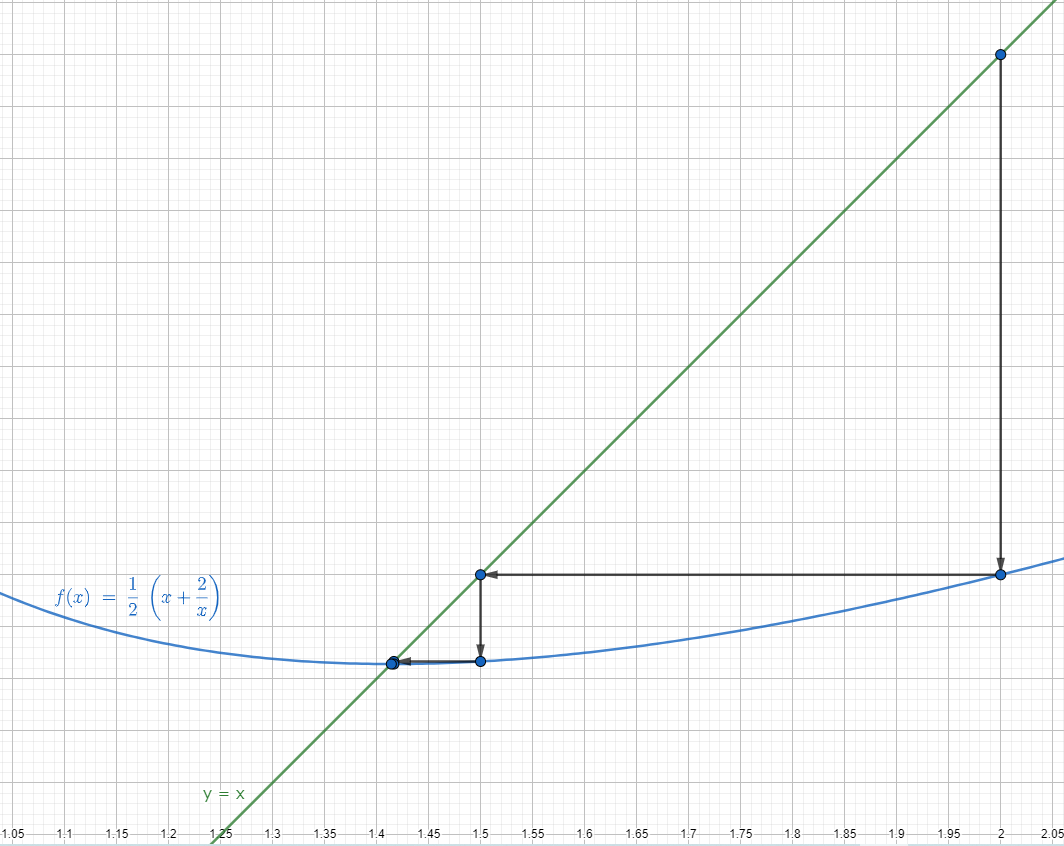
\includegraphics[width=0.45\textwidth]{f.PNG}\qquad
    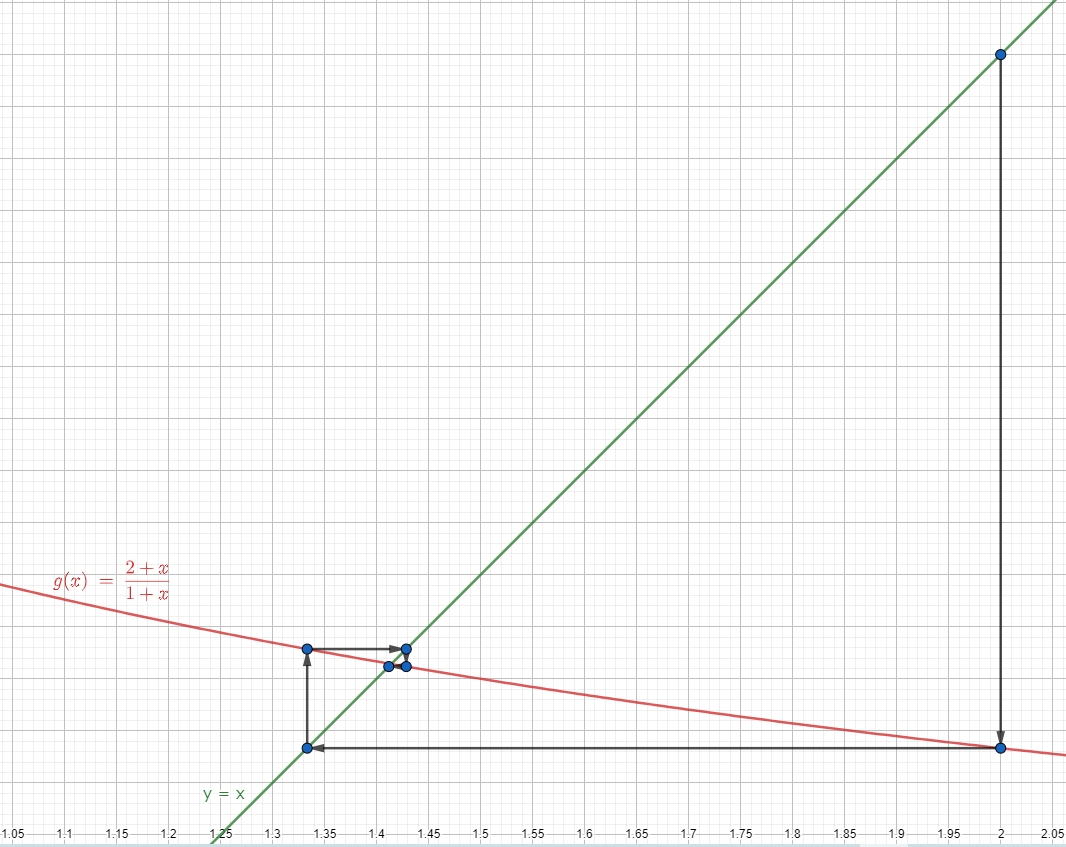
\includegraphics[width=0.45\textwidth]{g.PNG}
    \caption{The zig-zag paths of $f$ and $g$ in Exercise 24.}
    \label{fig:f}
\end{figure}

\paragraph{25.}
(a)
The tangent to the graph of $f$ at $(x_n,f(x_n))$ is $y=f'(x_n)(x-x_n)+f(x_n)$, which intersects with $x$-axis at $\left(x_n-\frac{f(x_n)}{f'(x_n)}\,,\,0\right)=(x_{n+1}\,,\,0)$.
\medskip

(b)
$x_1>\xi$. If $x_n>\xi$, then $f(x_n)>0$, so
\[
x_{n+1}=x_n-\frac{f(x_n)}{f'(x_n)}<x_n
\]
Also, by Theorem 5.10, there is $t\in(\xi,x_n)$ such that
\[
\frac{f(x_n)-f(\xi)}{x_n-\xi}=f'(t)<f'(x_n)
\]
since $f'$ is monotonically increasing by $f''(x)>0$. Rearranging, 
\[
x_{n+1}=x_n-\frac{f(x_n)}{f'(x_n)}>\xi
\]
Therefore, $\{x_n\}$ is monotonically decreasing and bounded below by $\xi$. Let the limit be $\xi'=\lim_{n\to\infty}x_n$, then since $\lim_{n\to\infty}x_{n+1}=\lim_{n\to\infty}x_n=\xi'$,
\[
\xi'=\xi'-\frac{f(\xi')}{f'(\xi')}
\]
so $f(\xi')=0$, which means $\xi'=\xi$.
\medskip

(c)
By Taylor's Theorem, there is $t_n\in(\xi,x_n)$ such that
\[
f(\xi)=f(x_n)+f'(x_n)(\xi-x_n)+\frac{f''(t_n)}{2}(\xi-x_n)^2
\]
Rearranging,
\[
x_{n+1}-\xi=x_n-\frac{f(x_n)}{f'(x_n)}-\xi=\frac{f''(t_n)}{2f'(x_n)}(x_n-\xi^2)
\]

(d)
\[
x_{n+1}-\xi\leq\frac{1}{A}\left[A(x_n-\xi)\right]^2
\]
The inequality holds for $n=1$. If it holds for $n=k$, so
\[
0\leq x_{k+1}-\xi\leq\frac{1}{A}\left[A(x_1-\xi) \right]^{2^n}
\]
then $x_{k+2}-\xi\geq0$ by (b), and
\[
x_{k+2}-\xi\leq A(x_{k+1}-\xi)^2\leq\frac{1}{A}\left[A(x_1-\xi)\right]^{2^{k+1}}
\]
so by induction, the inequality holds for every $n$.

The algorithms in Exercise 3.16 and 3.18 are Newton's methods applied on $x_n^2-\alpha$ and $x_n^p-\alpha$.
\medskip

(e)
$g(x)=x$ is equivalent to $f(x)=0$, so finding a fixed point of $g$ is finding the root of $f(x)$.
\[
g'(x)=1-\frac{\left[f'(x) \right]^2-f(x)f''(x)}{\left[f'(x) \right]^2}=\frac{f(x)f''(x)}{\left[f'(x) \right]^2}\leq\frac{f(x)M}{\delta^2}\to0
\]
as $x\to\xi$.
\medskip

(f)
\[
x_{n+1}=x_n-\frac{{x_n}^{\frac{1}{3}}}{\frac{1}{3}x_n^{-\frac{2}{3}}}=-2x_n
\]
so $\{x_n\}$ is an alternating sequence such that $\{|x_n|\}\to\infty$ as $n\to\infty$.

\paragraph{26.}
Let $x_0=a+\frac{1}{2A}$. For $a\leq x\leq x_0$,
\[
\left|\frac{f(x)-f(a)}{x-a} \right|=\left|f'(t) \right|\leq M_1
\]
where $t\in(a,x)\in(a,x_0)$. Rearranging,
\[
|f(x)|\leq M_1(x-a)\leq M_1(x_0-a)\leq AM_0(x_0-a)=\frac{M_0}{2}
\]
since $M_0$ is the least upper bound of $|f(x)|$, we have $M_0\leq\frac{M_0}{2}$, which means $M_0=0$, so $f(x)=0$ on $[a,a+\frac{1}{2A}]$. Repeat the process for finite steps, we have $f(x)=0$ on $[a,b]$.

\paragraph{27.}
Let $f(x)=y_2(x)-y_1(x)$, then $f$ is differentiable on $[a,b]$, and $f(a)=c-c=0$. If the inequality holds, then
\[
|f'(x)|=|y_2'-y_1'|=|\phi(x,y_2)-\phi(x,y_1)|\leq A|y_2-y_1|=A|f(x)|
\]
so by Exercise 26,\; $f(x)=0$, which means $y_2=y_1$, the solution is unique.

Consider $f(x)$ which is the solution of $y'=\sqrt{y}$ and $y(0)=0$. Since $y'=\sqrt{y}\geq0$, $y$ is monotonically increasing. Let $a$ be the real number such that $f(x)=0$ for $0\leq x\leq a$ and $f(x)>0$ for $x>a$. Let $F(x)=\sqrt{f(x)}$, then $F'(x)=\frac{f'(x)}{2\sqrt{f(x)}}=\frac{1}{2}$, so $F(x)=\frac{1}{2}(x+c)$, and $f(x)=\frac{(x+c)^2}{4}$. Since $f(a)=0$, we have $c=-a$. So the solution is 
\[
f(x)=\begin{cases}
0\quad & 0\leq x\leq a\\
\frac{(x-a)^2}{4}\quad & x>a
\end{cases}
\]
where $a$ can be arbitrary.

\paragraph{28.}
\textit{statement:}
Let $\pmb{\phi}$ be a vector-valued function in $R^k$ defined on a $(k+1)$-cell, given by $a\leq x\leq b$,\; $\alpha_j\leq y_j\leq \beta_j$. If there is a constant $A$ such that
\[
|\pmb\phi(x,\V{y}_2)-\pmb\phi(x,\V{y}_1) |\leq A|\V{y}_2-\V{y}_1|
\]
then the initial-value problem
\[
\V{y}'=\pmb{\phi}(x,\V{y}),\quad \V{y}(a)=\V{c}
\]
has at most one solution.
\medskip

\textit{proof:}
The result in Exercise 26 holds for vector-valued function since by Theorem 5.19,
\[
|\V{f}(x)-\V{f}(a)|\leq|\V{f}'(t)|(x-a)\leq M_1(x_0-a)\leq AM_0(x_0-a)
\]
and the other parts of the proof remain the same as Exercise 26.

Let $\V{f}=\V{y}_2(x)-\V{y}_1(x)$ where $\V{y}_2,\,\V{y}_1$ are the solutions of the initial-value problem, then the proof is the same as Exercise 27, except all the functions are vector-valued. So $\V{y}_2=\V{y}_1$, the solution is unique.

\paragraph{29.}
Let $\V{y}=(y_1,\cdots,y_k)$ and $\V{g}=(g_1,\cdots,g_k)$ be vectors in $R^k$. Let $\pmb\phi$ be a function form $R^{k+1}$ to $R^k$ defined as 
\[
\pmb\phi(x,\V{y})=(y_2,\cdots,y_k,f(x)-\V{g}\cdot\V{y})
\]
If $y_j=y^{(j-1)}$ for $1\leq j\leq k$, then
\[
y_j'=y^{(j)}=y_{j+1}\quad\textit{for $1\leq j\leq k-1$}\]
\[y_k'=y^{(k)}=f(x)-\sum_{j=1}^k g_j(x)y^{j-1}=f(x)-\sum_{j=1}^k g_j(x)y_j=f(x)-\V{g}\cdot\V{y} \]
\[
y^{(j-1)}(a)=y_j(a)=c_j\quad\textit{for $1\leq j\leq k$}
\]
so the initial-value problem given is equivalent to
\[
\V{y}'=\pmb\phi(x,\V{y}),\quad \V{y}(a)=\V{c}
\]
$g_1,\cdots,g_k$ are continuous real function on the compact space $[a,b]$, so $|g_j|$ is bounded, which means $|\V{g}|$ is bounded. Let $|\V{g}|\leq M$, and let $A=\sqrt{1+M^2}$, then
\begin{equation*}
    \begin{split}
        |\pmb\phi(x,\V{y}_b)-\pmb\phi(x,\V{y}_a)| & =\sqrt{\sum_{j=2}^k(y_{bj}-y_{aj})^2+|\V{g}\cdot(\V{y}_b-\V{y}_a)|^2}\\
        & \leq \sqrt{|\V{y}_b-\V{y}_a|^2+|\V{g}|^2|\V{y}_b-\V{y}_a|^2 }\\
        & =\sqrt{1+|\V{g}|^2}|\V{y}_b-\V{y}_a|\\
        & \leq A|\V{y}_b-\V{y}_a|
    \end{split}
\end{equation*}
so by Exercise 28, the solution is unique.







\end{document}
